
\section{解读：族的拉回与态射的纤维}

\textbf{10.3.1.\ 族的拉回。}\quad 在给出任何定义之前，我们先来看一个非正式的启发性例子。考虑 $xy$-平面中由 $t$ 参数化的「曲线族」
\[
y^2=x^3+tx.
\]
翻译成概形的语言：考虑
\[
\Spec k[x,y,t]/(y^2-x^3-tx)\longrightarrow\Spec k[t].
\]
如果我们经由 $uv=t$ 把这个族「拉回」到 $uv$-平面上，便得到族 $y^2=x^3+uvx$。如果我们不这样做，而是取 $t=3$，便得到曲线 $y^2=x^3+3x$，我们把它解读为原族在 $t=3$ 上方的\trFiber。你或许已经注意到这些构造背后潜藏的\trFiberProduct：
\[
\begin{tikzcd}[row sep=2.3em, column sep=2.4em]
\Spec k[x,y,u,v]/(y^2-x^3-uvx) \ar[r] \ar[d] & \Spec k[x,y,t]/(y^2-x^3-tx) \ar[d] \\
\Spec k[u,v] \ar[r, "uv\mapsto t"'] & \Spec k[t]
\end{tikzcd}
\]
以及
\[
\begin{tikzcd}[row sep=2.3em, column sep=2.4em]
\Spec k[x,y]/(y^2-x^3-3x) \ar[r] \ar[d] & \Spec k[x,y,t]/(y^2-x^3-tx) \ar[d] \\
\Spec k \ar[r, "3\mapsto t"'] & \Spec k[t]
\end{tikzcd}
\]
现在我们把这一切正式化。

设 $Y\to Z$ 是一个\trMorphism。我们把它解读为「由\textbf{\trBaseScheme{}}（base scheme）（或者干脆就叫\textbf{基}（base））$Z$ 参数化的一个概形族」。此时，若再给定另一个\trMorphism{} $\psi\colon X\to Z$，我们就把诱导出的映射 $X\times_Z Y\to X$ 解读为「拉回族」（见图~\ref{fig:pulled-back-family}）。
\[
\begin{tikzcd}[row sep=2.3em, column sep=3.4em]
X\times_Z Y \ar[r] \ar[d, "\text{拉回族}"'] & Y \ar[d, "\text{族}"] \\
X \ar[r, "\psi"'] & Z
\end{tikzcd}
\]

\begin{figure}[htbp]
\centering
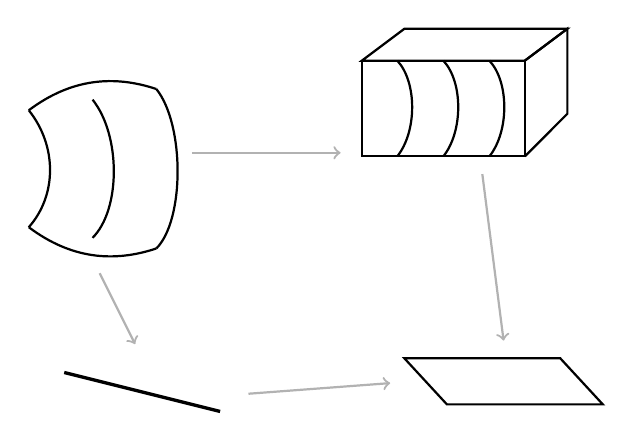
\begin{tikzpicture}[scale=0.9]
  \draw[thick] (0.0,0.4) .. controls (0.4,-0.1) and (0.4,-0.8) .. (0.0,-1.25);
  \draw[thick] (0.9,0.55) .. controls (1.3,0.05) and (1.3,-1.0) .. (0.9,-1.4);
  \draw[thick] (1.8,0.7) .. controls (2.2,0.2) and (2.2,-1.15) .. (1.8,-1.55);
  \draw[thick] (0.0,0.4) .. controls (0.6,0.85) and (1.2,0.9) .. (1.8,0.7);
  \draw[thick] (0.0,-1.25) .. controls (0.6,-1.7) and (1.2,-1.75) .. (1.8,-1.55);
  \begin{scope}[shift={(4.7,0.1)}]
    \draw[thick] (0,1.0) -- (2.3,1.0) -- (2.9,1.45) -- (0.6,1.45) -- cycle;
    \draw[thick] (2.3,1.0) -- (2.9,1.45) -- (2.9,0.25) -- (2.3,-0.35);
    \draw[thick] (0,1.0) -- (0,-0.35) -- (2.3,-0.35) -- (2.3,1.0);
    \draw[thick] (0.5,1.0) .. controls (0.78,0.7) and (0.78,0.0) .. (0.5,-0.35);
    \draw[thick] (1.15,1.0) .. controls (1.43,0.7) and (1.43,0.0) .. (1.15,-0.35);
    \draw[thick] (1.8,1.0) .. controls (2.08,0.7) and (2.08,0.0) .. (1.8,-0.35);
  \end{scope}
  \draw[very thick] (0.5,-3.3) -- (2.7,-3.85);
  \draw[thick] (5.3,-3.1) -- (7.5,-3.1) -- (8.1,-3.75) -- (5.9,-3.75) -- cycle;
  \draw[gray!60,thick,->] (2.3,-0.2) -- (4.4,-0.2);
  \draw[gray!60,thick,->] (1.0,-1.9) -- (1.5,-2.9);
  \draw[gray!60,thick,->] (6.4,-0.5) -- (6.7,-2.85);
  \draw[gray!60,thick,->] (3.1,-3.6) -- (5.1,-3.45);
\end{tikzpicture}
\caption{拉回族的一幅图。（依原书手绘图重绘。）}\label{fig:pulled-back-family}
\end{figure}

我们有时说：$X\times_Z Y$ 是 $Y$ 的\textbf{\trSchemeTheoreticPreimage{}}（scheme-theoretic preimage）（或概形论拉回（scheme-theoretic pullback），或概形论逆像（scheme-theoretic inverse image），或逆像概形（inverse image scheme））。（我们即将展开的关于\trFiber{}的讨论，或许能给出这样叫的些许动机。）正因如此，\trFiberProduct{}常被称作\textbf{\trBaseChange}、\textbf{\trChangeOfBase{}}（change of base）或\textbf{\trPullback}。除了 \S1.2.7 中给\trCartesianDiagram{}起的种种名字之外，在代数几何中它还常被称作\textbf{\trBaseChangeDiagram{}}（base change diagram）或\textbf{拉回图}（pullback diagram）；而 $X\times_Z Y\to X$ 称作 $Y\to Z$ 经 $\psi$ 的\textbf{\trPullback}，$X\times_Z Y$ 称作 $Y$ 经 $\psi$ 的\textbf{\trPullback}。谈论 $X\times_Z Y$ 时，人们常说「在 $X$ 之上」（over $X$）或「在 $X$ 上方」（above $X$）——当 $X$ 是 $Z$ 的一个\trLocally\trClosed\trSubscheme{}时尤其如此。（顺带一提：\trSchemeTheoreticPreimage{}总是有意义的，而\trSchemeTheoreticImage{}这一观念却在某种意义上成问题，见 \S9.4.1 的讨论。）

\textbf{10.3.2.\ 态射的\trFiber。}\quad （如果你做过\mbox{练习~8.3.J}——有限\trMorphism{}有有限的\trFiber——你不会觉得下面的讨论出人意料。）\trPullback{}的一个特殊情形，便是\trMorphism{}的\trFiber{}这一观念。我们用拓扑空间范畴中的\trFiber{}观念来引入它。

\textbf{10.3.A.（练习）}\quad 证明：若 $Y\to Z$ 是\trTopologicalSpace{}之间的一个\trContinuousMap，而 $X$ 是 $Z$ 的一点 $\mathsf{p}$，则 $Y$ 在 $\mathsf{p}$ 之上的\trFiber{}（即集合论的\trFiber，配备诱导拓扑）自然地认同于 $X\times_Z Y$。

更一般地，对任意 $\pi\colon X\to Z$，$X\times_Z Y\to X$ 在 $X$ 的一点 $\mathsf{p}$ 之上的\trFiber，自然地认同于 $Y\to Z$ 在 $\pi(\mathsf{p})$ 之上的\trFiber。

\textbf{10.3.3.}\ \emph{\trhDefinition{}}\quad 受拓扑学启发，我们回到概形的\trCategory。设 $\mathsf{p}\to Z$ 是一点的包含态射（该点未必\trClosed）。更确切地说，若 $\mathsf{p}$ 是\trResidueField{}为 $K$ 的一点，考虑把 $\Spec K$ 送到 $\mathsf{p}$ 的映射 $\Spec K\to Z$，并连同\trResidueField{}的自然同构。此时，若 $g\colon Y\to Z$ 是任意\trMorphism，则 $\mathsf{p}$ 的\trSchemeTheoreticPreimage{}称作 $g$ \textbf{在 $\mathsf{p}$ 上方}（above $\mathsf{p}$）的\textbf{概形论\trFiber}（scheme-theoretic fiber）（或 \emph{fibre}），记作 $g^{-1}(\mathsf{p})$。若 $Z$ \trIrreducible，则 $Z$ 的\trGenericPoint{}上方的概形论\trFiber{}称作（$g$ 的）\textbf{一般\trFiber}（generic fiber）。在含 $\mathsf{p}$ 的一个\trAffine\trOpenSubscheme{} $\Spec\scr{A}$ 中，$\mathsf{p}$ 对应于某个\trPrimeIdeal{} $\mathfrak{p}$，而\trMorphism{} $\Spec K\to Z$ 对应于环映射 $\scr{A}\to\scr{A}_{\mathfrak{p}}/\mathfrak{p}\scr{A}_{\mathfrak{p}}$。这是\trLocalization{}与\trClosedEmbedding{}的\trComposition，因而可以由上面的技巧算出。（注意：由\mbox{练习~10.2.H}，$\mathsf{p}\to Z$ 是一个\trMonomorphism。）

\textbf{10.3.B.（练习）}\quad 证明：$X\to Y$ 在一点 $\mathsf{p}$ 上方的概形论\trFiber{}的底拓扑空间，自然地认同于 $X\to Y$ 在 $\mathsf{p}$ 上方的拓扑\trFiber。

\textbf{10.3.C.（练习：练习~10.3.A 的类比）}\quad 设 $\pi\colon Y\to Z$ 与 $\tau\colon X\to Z$ 是\trMorphism，而 $\mathsf{p}\in X$ 是一点。证明：$X\times_Z Y\to X$ 在 $\mathsf{p}$ 之上的\trFiber{}（同构于）$\pi\colon Y\to Z$ 在 $\tau(\mathsf{p})$ 之上的\trFiber{}到 $\mathsf{p}$ 的\trBaseChange。

\begin{figure}[htbp]
\centering
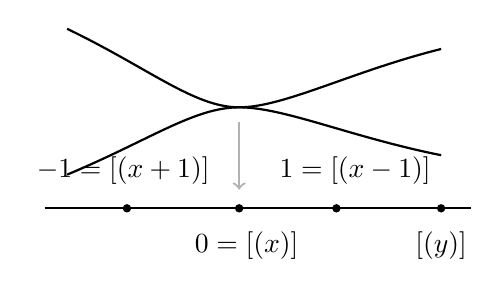
\begin{tikzpicture}[scale=0.95]
  \draw[thick] (-2.3,1.05) .. controls (-1.2,0.52) and (-0.6,0.0) .. (0,0)
               .. controls (0.6,0.0) and (1.5,0.48) .. (2.7,0.78);
  \draw[thick] (-2.3,-0.9) .. controls (-1.2,-0.44) and (-0.6,0.0) .. (0,0)
               .. controls (0.6,0.0) and (1.5,-0.4) .. (2.7,-0.64);
  \draw[thick] (-2.6,-1.35) -- (3.1,-1.35);
  \draw[gray!60,thick,->] (0.0,-0.2) -- (0.0,-1.1);
  \fill (-1.5,-1.35) circle (1.6pt);
  \fill (0.0,-1.35) circle (1.6pt);
  \fill (1.3,-1.35) circle (1.6pt);
  \fill (2.7,-1.35) circle (1.6pt);
  \node at (-1.55,-0.85) {$-1=[(x+1)]$};
  \node at (1.55,-0.85) {$1=[(x-1)]$};
  \node at (0.1,-1.85) {$0=[(x)]$};
  \node at (2.7,-1.85) {$[(y)]$};
\end{tikzpicture}
\caption{由 $y\mapsto y^2$ 给出的映射 $\mathbb{C}\to\mathbb{C}$（参看图~\ref{fig:parabola-map}）。（依原书手绘图重绘。）}\label{fig:y-squared-map}
\end{figure}

\textbf{10.3.4.}\ \emph{\trhExample{}（在好几个层面上都富有启发）。}\quad 考虑 $\mathbb{Q}$ 上\trParabola{} $y^2=x$ 到 $x$-轴的\trProjection，对应的环映射为 $\mathbb{Q}[x]\to\mathbb{Q}[y]$，$x\mapsto y^2$。如果 $\mathbb{Q}$ 让你不安，就把它换成你最喜欢的\trField，看看会发生什么。（你应当看看图~\ref{fig:y-squared-map}——它是图~\ref{fig:parabola-map} 中那条\trParabola{}的翻转版本——并琢磨该怎样修改它，才能反映我们在这里洞见到的东西。）把 $\mathbb{Q}[y]$ 写作 $\mathbb{Q}[x,y]/(y^2-x)$，会便于我们解读这个\trMorphism。

(i)~于是 $1$ 的原像是两个点：
\[
\begin{aligned}
\Spec\mathbb{Q}[x,y]/(y^2-x)\otimes_{\mathbb{Q}[x]}\mathbb{Q}[x]/(x-1)&\cong\Spec\mathbb{Q}[x,y]/(y^2-x,\,x-1)\\
&\cong\Spec\mathbb{Q}[y]/(y^2-1)\\
&\cong\Spec\mathbb{Q}[y]/(y-1)\amalg\Spec\mathbb{Q}[y]/(y+1).
\end{aligned}
\]
(ii)~$0$ 的原像是一个非既约的点：
\[
\Spec\mathbb{Q}[x,y]/(y^2-x,\,x)\cong\Spec\mathbb{Q}[y]/(y^2).
\]
(iii)~$-1$ 的原像是一个既约的点，但「在\trBaseField{}上大小为 $2$」：
\[
\begin{aligned}
\Spec\mathbb{Q}[x,y]/(y^2-x,\,x+1)&\cong\Spec\mathbb{Q}[y]/(y^2+1)\\
&\cong\Spec\mathbb{Q}[i]\\
&=\Spec\mathbb{Q}(i).
\end{aligned}
\]
(iv)~\trGenericPoint{}的原像又是一个既约的点，但「在\trResidueField{}上大小为 $2$」，我们这就来验证：
\[
\Spec\mathbb{Q}[x,y]/(y^2-x)\otimes_{\mathbb{Q}[x]}\mathbb{Q}(x)\cong\Spec\mathbb{Q}[y]\otimes_{\mathbb{Q}[y^2]}\mathbb{Q}(y^2),
\]
亦即（非正式地说）「$y$ 的多项式们除以 $y^2$ 的多项式们」所得之环的 Spec。稍加思考便能明白：在这个环里，你可以把\emph{任何一个} $y$ 的多项式都取逆——因为若 $f(y)$ 是任意一个 $y$ 的多项式，则
\[
\frac{1}{f(y)}=\frac{f(-y)}{f(y)f(-y)},
\]
而右边的分母是 $y^2$ 的多项式。于是
\[
\mathbb{Q}[x,y]/(y^2-x)\otimes_{\mathbb{Q}[x]}\mathbb{Q}(x)\cong\mathbb{Q}(y),
\]
这是 $\mathbb{Q}(x)$ 的一个 $2$ 次\trFieldExtension（注意 $\mathbb{Q}(x)=\mathbb{Q}(y^2)$）。

（你或许还想把 $\mathbb{A}^1_{\mathbb{Q}}$ 的其他一些点的原像也走一遍，比如 $[(x^3-4)]$ 与 $[(x^2-2)]$。）

请注意下面这个有趣的事实。在全部四种情形里，原像的个数都可以解读为 $2$，只是「数到二」的方式各有不同：你可以去数点（如 $1$ 的原像那样）；你可能得到非既约的行为（如 $0$ 的原像那样）；又或者你会得到一个 $2$ 次的\trFieldExtension（如 $-1$ 或\trGenericPoint{}的原像那样）。无论哪种情形，该\trFiber{}都是一个\trAffine\trScheme，它作为该点的\trResidueField{}上的\trVectorSpace{}的\trDimension{}为 $2$。有\trNumberTheory{}背景的读者或许以前就见过这种行为。我们将在 \S16.3.10 重访这个例子。它将成为某一类非常重要的\trMorphism{}（\trFinite\trFlat\trMorphism；见注记~24.3.8 与 \S24.3.12）的典型症候。

如果做得到的话，试着为这个\trMorphism{}画一幅图，好让你为个中情形发展出一套图形速记。图~\ref{fig:y-squared-map} 中那条\trParabola{}是很好的第一近似，但你还会想以某种方式描绘出 (iii) 与 (iv) 的特异之处。

\textbf{10.3.5.}\ \emph{\trhRemark{}：有限\trMorphism{}有有限的\trFiber。}\quad 如果你还没有做过\mbox{练习~8.3.J}（有限\trMorphism{}有有限的\trFiber），现在正是做的良机——以你如今的积累，你会发现它直截了当得多。

\textbf{10.3.D.（练习：对有较多算术背景的读者尤为重要）}\quad $\Spec\mathbb{Z}[i]\to\Spec\mathbb{Z}$ 在素数 $(p)$ 上方的概形论\trFiber{}是什么？你的答案将依赖于 $p$，共有四种情形，与例~10.3.4 的四种情形一一对应。（你能画出图来吗？）

\textbf{10.3.E.（练习）}\quad （这道练习会让你练习在某个不是域的东西上作\trFiberProduct。）考虑概形之间的\trMorphism{} $X=\Spec k[t]\to Y=\Spec k[u]$，对应的环映射为 $k[u]\to k[t]$，$u\mapsto t^2$，其中 $\operatorname{char}k\neq 2$。证明：$X\times_Y X$ 有两个\trIrreducibleComponent。（若 $\operatorname{char}k=2$ 会怎样？线索见\mbox{练习~10.5.A}。）

\textbf{10.3.6.}\ \emph{\trBlowup{}初窥。}

\textbf{10.3.F.（重要的具体练习）}\quad （这里的讨论立即可推广到 $\mathbb{A}^n_k$。）如下定义 $\mathbb{A}^2_k\times_k\mathbb{P}^1_k$ 的一个\trClosedSubscheme{} $\mathrm{Bl}_{(0,0)}\mathbb{A}^2_k$（见图~\ref{fig:blowup-first-example}）。若 $\mathbb{A}^2_k$ 上的\trCoordinate{}是 $x$、$y$，而 $\mathbb{P}^1_k$ 上的射影\trCoordinate{}是 $u$、$v$，则这个子概形在 $\mathbb{A}^2_k\times_k\mathbb{P}^1_k$ 中由单个方程 $xv=yu$ 切出。（你不妨这样来解读 $\mathrm{Bl}_{(0,0)}\mathbb{A}^2_k$：$\mathbb{P}^1_k$ 参数化了过原点的诸直线。这个\trBlowup{}对应的有序对（点 $\mathsf{p}$，直线 $\ell$），恰是那些使 $(0,0)$ 与 $\mathsf{p}$ 都落在 $\ell$ 之上的对。）请描述\trMorphism{} $\mathrm{Bl}_{(0,0)}\mathbb{A}^2_k\to\mathbb{P}^1_k$ 在 $\mathbb{P}^1_k$ 的每个\trClosedPoint{}上方的\trFiber。证明：\trMorphism{} $\mathrm{Bl}_{(0,0)}\mathbb{A}^2_k\to\mathbb{A}^2_k$ 在 $(0,0)\in\mathbb{A}^2_k$ 之外是一个\trIsomorphism。证明：$(0,0)$ 上方的\trFiber{}是一个\trEffectiveCartierDivisor（\S9.5.1：由单个方程局部切出、且该方程不是\trZerodivisor{}的\trClosedSubscheme）。它称作\textbf{\trExceptionalDivisor{}}（exceptional divisor）。我们将在第~22 章讨论\trBlowup。这个具体的例子还将在 \S22.1 的启发性例子以及\mbox{练习~20.2.D}中登场。

\begin{figure}[htbp]
\centering
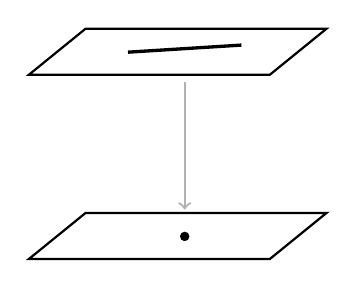
\begin{tikzpicture}[scale=0.9]
  \draw[thick] (-0.2,0.1) -- (3.2,0.1) -- (4.0,0.75) -- (0.6,0.75) -- cycle;
  \draw[very thick] (1.2,0.42) -- (2.8,0.52);
  \begin{scope}[shift={(0,-2.6)}]
    \draw[thick] (-0.2,0.1) -- (3.2,0.1) -- (4.0,0.75) -- (0.6,0.75) -- cycle;
    \fill (2.0,0.42) circle (1.9pt);
  \end{scope}
  \draw[gray!60,thick,->] (2.0,0.0) -- (2.0,-1.8);
\end{tikzpicture}
\caption{\trBlowup{}的第一例。（依原书手绘图重绘。）}\label{fig:blowup-first-example}
\end{figure}

我们还没有讨论过正则性，但这里有一番「挥手」式的粗略论证，暗示 $\mathrm{Bl}_{(0,0)}\mathbb{A}^2_k$ 是「\trSmooth」的：$\mathbb{P}^1$ 的任何一个\trStandardOpenSet{} $\mathsf{U}_i\subset\mathbb{P}^1$ 之上的原像都\trIsomorphic{}于 $\mathbb{A}^2$。于是：「这个\trBlowup{}是这样一台外科手术：把\trSmooth{}曲面 $\mathbb{A}^2_k$ 取来，切掉一个点，再缝回去一个 $\mathbb{P}^1$，而且缝成的结果仍是另一张\trSmooth{}曲面。」

\textbf{10.3.7.\ 泛\trFiber、一般\trFiber{}与\trGenericallyFinite{}\trMorphism。}\quad 「一般\trFiber」与「泛\trFiber」这两个说法，平行于「\trGenericPoint」与「\trGeneralPoint」的说法（定义~3.6.11）。\footnote{译注：本译本把 general／generic 分别定译为「泛／一般」，与定义~3.6.11 中「\trGeneralPoint（general point）／\trGenericPoint（generic point）」的既有口径一致；一部分中文文献的习惯（把 generic 译作「泛」）与此正好相反，阅读时请留意。}设 $\pi\colon X\to Y$ 是概形之间的\trMorphism。当人们说 $\pi$ 的\textbf{泛\trFiber}（general fiber）（或\emph{一个}泛\trFiber）具有某条性质时，意思是：存在\trDense{}的\trOpenSubset{} $\mathsf{U}\subset Y$，使得 $\mathsf{U}$ 中任何一点上方的诸\trFiber{}都有这条性质。

而当人们说 $\pi\colon X\to Y$ 的\emph{一般\trFiber}（定义~10.3.3）时，这话隐含着 $Y$ \trIrreducible，并且指的是\trGenericPoint{}上方的那一个\trFiber。\emph{泛\trFiber}与\emph{一般\trFiber}不是一回事！显然，若某件事对泛\trFiber{}成立，那它对一般\trFiber{}也成立；但反过来并不总是真。然而在好的情势下，反过来也可以成立——一般\trFiber{}的性质可以扩展到一片货真价实的\trOpen\trNeighborhood{}上。例如，若 $Y$ \trIrreducible{}且\trNoetherian，而 $\pi$ 是\trFiniteType{}的，则由\trChevalley{}定理~8.4.2：若 $\pi$ 的一般\trFiber{}为空（相应地，非空），则泛\trFiber{}为空（相应地，非空）。

若 $\pi\colon X\to Y$ 是\trFiniteType{}的，则当 $\pi$ 经\trBaseChange{}到每个\trIrreducibleComponent{}的\trGenericPoint{}之后是有限的，我们称 $\pi$ \textbf{\trGenericallyFinite{}}（generically finite）（或者，由\cref{ex:quasifinite-to-field-finite}，等价地：若 $Y$ 的每个\trIrreducibleComponent{}的\trGenericPoint{}的原像都是有限集）。（\trGenericallyFinite{}性这一观念可以在更一般的情势下定义；见 [Stacks, tag 073A]。）

\textbf{10.3.G.（练习：「\trGenericallyFinite{}」通常意味着「泛有限」）}\quad 设 $\pi\colon X\to Y$ 是局部\trNoetherian{}概形之间的一个\trAffine、\trFiniteType、\trGenericallyFinite{}的\trMorphism，且 $Y$ \trReduced。证明：$Y$ 的每个\trGenericPoint{}都有一个\trOpen\trNeighborhood，在其上 $\pi$ 实际上是有限的。（这些假设可以大幅削弱；见 [Stacks, tag 02NW]。）提示：化归到 $Y=\Spec B$（$B$ 是一个\trIntegralDomain）的情形。此时 $X$ 是仿射的，比如说 $X=\Spec\scr{A}$。写出 $\scr{A}=B[x_1,\dots,x_n]/I$。由假设，$\scr{A}\otimes_B K(B)$ 是一个\trFinite{} $K(B)$-\trModule（\trFiniteDimensional{}\trVectorSpace），故存在\trMonicPolynomial{} $f_i(t)\in K(B)[t]$，使得在 $\scr{A}\otimes_B K(B)$ 中 $f_i(x_i)=0$。设 $b$ 为诸 $f_i(x)$ 的系数中出现的（有限多个）分母之乘积。把 $B$ 换成 $B_b$，论证你可以假定 $f_i(t)\in B[t]$。于是在 $\scr{A}\otimes_B K(B)$ 中 $f_i(x_i)=0$，这意味着 $f_i(x_i)$ 被 $B$ 的某个非零元\trAnnihilate。再把 $B$ 换成它在这 $n$ 个非零元之乘积处的\trLocalization（「把 $\Spec B$ 进一步收缩」），论证在 $\scr{A}$ 中 $f_i(x_i)=0$。然后得出结论。

\textbf{10.3.8.}\ \extrahard\ \textbf{\trFinitelyPresented{}族（\trMorphism）是某些格外好的族的局部拉回。}\quad 假如你是个硬汉，而且觉得\trNoetherian{}环让你脸上无光，那么下面这道练习可以用来把种种结果从\trNoetherian{}情形推广到\trLocally\trFinitelyPresented{}的情势。\mbox{练习~10.3.I}——它是\trChevalley{}定理~8.4.2 的一个推广——就是个好例子。

\textbf{10.3.H.（练习）}\quad 设 $\pi\colon X\to\Spec B$ 是一个\trFinitelyPresented\trMorphism。证明：存在形如下式的\trBaseChangeDiagram{}：
\[
\begin{tikzcd}[row sep=2.3em, column sep=4.2em]
X \ar[r] \ar[d, "\pi"'] & X' \ar[d, "\pi'"] \\
\Spec B \ar[r, "\rho"'] & \Spec\mathbb{Z}[x_1,\dots,x_N]
\end{tikzcd}
\]
其中 $N$ 是某个整数，而 $\pi'$ \trFinitelyPresented{}（＝\trFiniteType，因为靶是\trNoetherian{}的；见 \S8.3.13）。于是，每个\trFinitelyPresented\trMorphism{}都（在基上）局部地是某个映入\trNoetherian{}概形的\trFiniteType\trMorphism{}的\trPullback。从而，凡是对\trNoetherian{}概形证明了的、并且在\trBaseChange{}下稳定的结论，都自动对映入任意概形的\trLocally\trFinitelyPresented\trMorphism{}成立。提示：先思考 $X$ 仿射的情形。若 $X=\Spec\scr{A}$，则 $\scr{A}=B[y_1,\dots,y_n]/(f_1,\dots,f_r)$。为 $f_i\in B[y_1,\dots,y_n]$ 的每一个系数选定一个变量 $x_i$。此时 $X'$ 是什么？接着考虑 $X$ 是两个交为\trAffine\trOpenSet{}的\trAffine\trOpenSet{}之并的情形。然后再考虑更一般的情形，直到你解出完整的问题。你需要用到\trFinitelyPresented{}定义中的每一个部分。（\mbox{练习~25.2.B} 推广了这条结果。）

\vkexsync{I}
\begin{exercise}[\trLocally\trFinitelyPresented\trMorphism{}的\trChevalley{}定理]\label{ex:chevalley-locally-finitely-presented}
\begin{enumerate}[label=(\alph*)]
  \item 设 $\scr{A}$ 是一个\trFinitelyPresented{}的 $B$-\trAlgebra（$B$ 未必\trNoetherian），于是 $\scr{A}=B[x_1,\dots,x_n]/(f_1,\dots,f_r)$。证明：$\Spec\scr{A}\to\Spec B$ 的\trImage{}是 $\Spec B$ 的\trLocally\trClosed{}子集的有限并。（提示：\mbox{练习~10.3.H}（较容易的仿射情形）。）
  \item 证明：若 $\pi\colon X\to Y$ 是一个\trQuasicompact{}的\trLocally\trFinitelyPresented\trMorphism，而 $Y$ 也\trQuasicompact，则 $\pi(X)$ 是\trLocally\trClosed{}子集的有限并。（仅供铁杆专家：[Gr-EGA, 0$_{\mathrm{III}}$, 9.1] 给出了局部可构造性（local constructibility）以及更一般情形下可构造性的定义。\trChevalley{}可构造性定理的普遍形式 [Gr-EGA, IV$_1$, 1.8.4] 说的是：\trLocally\trConstructible{}子集在\trFinitelyPresented{}映射下的\trImage{}也局部可构造。）
\end{enumerate}
\end{exercise}
